\chapter{Fundamentação Teórica}
\label{fundamentacao_teorica}
\section{Sistemas de VANTs}

Esta seção fornece uma visão geral dos conceitos fundamentais necessários para compreender os sistemas de VANT, seus mecanismos de controle e os princípios de coordenação em enxames. Começamos detalhando os principais componentes e classificações dos VANTs, seguido por uma discussão sobre estratégias de controle e, por fim, as arquiteturas de enxames.

\subsection{Principais componentes de um VANT}
Um VANT (Veículo Aéreo Não Tripulado) consiste em diversos componentes essenciais que possibilitam sua operação autônoma. Estes incluem:
\begin{itemize}
    \item \textbf{Estrutura do Drone:} O quadro (ou frame) de um drone é a estrutura física que serve como base para todos os seus componentes. Ele é responsável por suportar os motores, hélices, controladores de voo, baterias, sensores e demais módulos eletrônicos. Em geral, o frame é projetado para ser leve, rígido e resistente, a fim de garantir estabilidade e eficiência durante o voo.
    \item \textbf{Sistema de Propulsão:} Motores elétricos e hélices para UAVs de múltiplos rotores ou motores a combustão para drones de asa fixa de maior porte.
    \item \textbf{Controladora de Voo:}  É o componente central do drone responsável por interpretar os dados dos sensores (como giroscópios, acelerômetros, GPS e magnetômetros) e enviar comandos precisos aos motores para estabilizar e controlar o voo.
    \item \textbf{Computador embarcado:} Sistema de computação embarcada que realiza o processamento de dados oriundos dos sensores, do controlador de voô e da estação solo. Geralmente neste componente que ocorre a execução dos algoritmos de visão computacional essenciais para a navegação do drone. Neste componente que as decisões de alto nível são tomadas e repassadas a controladora de voo.
    \item \textbf{Sensores:} Unidades de Medição Inercial (IMU), GPS, LiDAR, câmeras e barômetros, que auxiliam na navegação, estabilidade e percepção do ambiente.
    \item \textbf{Sistema de Comunicação:} Links de dados para telemetria, controle e coordenação entre os agentes.
\end{itemize}

% Os UAVs podem ser classificados com base em:
% \begin{enumerate}
%     \item \textbf{Tamanho e Peso:} UAVs nano, micro, pequenos, médios e grandes.
%     \item \textbf{Nível de Autonomia:} Drones pilotados remotamente, semiautônomos e totalmente autônomos.
%     \item \textbf{Capacidades de Voo:} UAVs de asa fixa (maior autonomia), UAVs de rotores (capacidade de pairar) e UAVs híbridos.
% \end{enumerate}

%\noindent\textbf{TO-DO:} Criar Diagrama ilustrando os componentes que constituem um VANT, ou tirar foto do drone no Laboratorio

\subsection{Dinâmica de Voô de um Quadricoptero}
Neste trabalho a estrutura adotada para o drone será a de 4 motores, denominado quadricoptero ou \textit{quadcopter}. Este tipo de drone possui 6 (seis) graus de liberdade (DOF), sendo 3 rotacionais e 3 translacionais. A sua dinâmica pode ser modelada da seguinte forma: 
[$\omega_1,\omega_2,\omega_3 ,\omega_4]$ indicam a velocidade angular cada um dos motores. Os ângulos de euler denominados roll, pitch e yaw são indicados como $[\phi,\theta,\psi]$ respectivamente. Portanto o efeito aerodinâmico $u$ que cada velocidade $w_i$ tem na força de empuxo $f$ e nos ângulos de rotação é definido por:


\begin{align}
    u_f &= b(\omega_1^2 + \omega_2^2 + \omega_3^2 + \omega_4^2) \quad \text{[Empuxo Total]} \\
    u_\phi &= b \cdot L(\omega_4^2 - \omega_2^2) \quad \text{[Momento de Rolagem]} \\
    u_\theta &= b \cdot L(\omega_3^2 - \omega_1^2) \quad \text{[Momento de Arfagem]} \\
    u_\psi &= d(\omega_1^2 - \omega_2^2 + \omega_3^2 - \omega_4^2) \quad \text{[Momento de Guinada]}\\
    m\ddot{\mathbf{p}} &= -m\mathbf{g}+\mathbf{R}\cdot{u_f} \quad \text{[Dinâmica Translacional]}
    \end{align}
%
 
% \begin{equation}
%     u_f =b(\omega_1^2 +\omega_2^2 +\omega_3 ^2 +\omega_4 ^2)     
% \end{equation}
% \begin{equation}
%     u_\phi =b(\omega_1^2 +\omega_2^2 -\omega_3 ^2 -\omega_4 ^2)\\
% \end{equation}
% \begin{equation}
%     u_\theta =b(\omega_1^2 -\omega_2^2 +\omega_3 ^2 -\omega_4 ^2)\\
% \end{equation}
% \begin{equation}
%     u_\psi =b(\omega_1^2 -\omega_2^2 -\omega_3 ^2 +\omega_4 ^2)\\
% \end{equation}
  
%Onde $u_f,u_\phi,u_\theta$
Onde $b$ é o coeficiente de empuxo, $d$ é o coeficiente de arrasto, $L$ distância entre o centro de massa e o motor e $\mathbf{R}$ é matriz de rotação transformada de coordenadas. Para o drone realizar uma manobra, o seu sistema de controle de voô  deve ser capaz coordenar as velocidades dos rotores com o intuito de atingir o movimento (rotação e translação) esperado.

\begin{figure}[H]
\centering
\includegraphics[scale=0.5]{fig/uav_dynamics_3.png}   
\caption{Diagrama esquemático da dinâmica de um VANT com 4 motores}
%S\fonte{Elaborado pelo autor.}
\label{fig:dynamic_quadrotor}
\end{figure}


\subsection{Sistema de Controle de Voo}
Um sistema de controle de voo de UAV é o mecanismo central que mantém e ajusta a orientação de um drone durante o voo, gerenciando o yaw, pitch e roll. Esse sistema de controle depende do feedback dos sensores para comparar continuamente a atitude real com o estado desejado, efetuando correções rápidas para garantir a estabilidade. Dentre as principais estratégias existente para o controle de voo, abrangem técnicas clássicas até métodos avançados baseados em IA. 

\subsubsection{Controle PID}
Os controladores PID nos sistemas de voo utilizam da teoria clássica de controle, especialmente na análise no domínio da frequência das funções de transferência. Ao representar o comportamento dinâmico do UAV por meio de uma função de transferência, é possível estudar como o sistema responde a diferentes frequências. O controlador PID ajusta os ganhos proporcional, integral e derivativo para modelar a resposta em frequência, aprimorando a estabilidade e o desempenho do sistema. Esse processo de ajuste garante que a atitude do drone — seu roll, pitch e yaw — permaneça responsiva aos comandos de controle, minimizando ultrapassagens e oscilações. Em essência, o projeto do controlador PID aproveita os insights matemáticos obtidos a partir da resposta em frequência do sistema, possibilitando uma estratégia de controle precisa e robusta para manter um desempenho de voo ideal.
O sinal de controle de saída é matematicamente definido no domínio do tempo como:
\begin{equation}
    u(t) = K_p \, e(t) + K_i \int_0^t e(\tau) \, d\tau + K_d \, \frac{d}{dt} e(t)
\end{equation}
onde:
\begin{itemize}
    \item $u(t)$ é o comando de controle enviado aos atuadores.
    \item $e(t)$ é o erro entre o estado desejado e o real.
    \item $K_p$, $K_i$ e $K_d$ são os ganhos proporcional, integral e derivativo, respectivamente.
\end{itemize}
Aplicando a transformada de Laplace o sinal de controle no domínio da frequência torna-se:
\begin{equation}
    C(s) = K_p + \frac{K_i}{s} + K_d s
\end{equation}
\begin{figure}[H]
    \centering
\begin{center}
\begin{tikzpicture}[auto, node distance=1cm]

    % Nodes
    \node [sum] (sum) {$+$};
   \node [block, right=of sum] (controller) {$C(s) = K_p + \frac{K_i}{s} + K_d s$};
    \node [block, right=of controller] (quad) {$G(s) = \frac{1}{I s^2}$};
    \node [coordinate, right=of quad] (output) {};
    \node [coordinate, below=1.5cm of quad] (feedback) {};
    \node [coordinate, left=of sum] (input) {};

    % Arrows
    \draw [arrow] (input) -- node{\Large$R(s)$} (sum);
    \draw [arrow] (sum) -- (controller);
    \draw [arrow] (controller) -- node{\Large$u(t)$} (quad);
    \draw [arrow] (quad) -- node{\Large$Y(s)$} (output);
    \draw [arrow] (output) |- (feedback) -| node[pos=0.9, above]{\Large$-$} (sum);

\end{tikzpicture}
\end{center}
    \caption{Malha de controle fechada quadrotor}
    \fonte{Elaborado pelo autor.}
    \label{fig:malha_fechada_drone}
\end{figure}
Onde $G(s)$ representa a função transferência de malha aberta que modela a dinâmica do drone com 4 rotores, sendo $I$  momento de inércia sob os respectivos eixos. $R(s)$ indica a entrada de referência, ou seja, os ângulos roll,pitch e yaw desejados. $Y(s)$ representa a saída obtida a partir dos sensores IMU do drone, que são retroalimentados para computação do erro, ajustando a entrada do controlador.

%\noindent\textbf{Sugestão de Ilustração:} Diagrama em blocos de um sistema de controle de voo de UAV usando PID, mostrando comandos de entrada, loops de feedback e resposta dos atuadores.

\section{Enxame de VANTs}
\subsection{Definição }
Um \textbf{enxame de VANTs (Veículos Aéreos Não Tripulados)} refere-se a um grupo coordenado de drones autônomos ou semiautônomos que colaboram de forma distribuída para atingir um objetivo comum. Esses sistemas inspiram-se frequentemente em comportamentos coletivos observados na natureza, como colônias de insetos sociais, e destacam-se por sua capacidade de operar de maneira cooperativa, robusta e eficiente \cite{brambilla2013swarm, chung2018survey}.

Entre as propriedades fundamentais que caracterizam um enxame de VANTs, destacam-se:
\begin{itemize}
    \item \textbf{Arquitetura}: Esta propriedade define o local no qual as decisões do exame são processadas. As principais arquiteturas são: centralizada, descentralizada e híbrida \cite{bayndir2016review}.
    \item \textbf{Escalabilidade}: Diz respeito à capacidade do sistema de manter sua eficiência à medida que o número de agentes no enxame aumenta. Um sistema escalável é capaz de coordenar ações com dezenas ou centenas de UAVs sem comprometer o desempenho geral  \cite{chung2018survey}.
    \item \textbf{Adaptabilidade}: Representa a habilidade do enxame de reagir a mudanças no ambiente, como a presença de obstáculos, a movimentação de alvos ou a introdução de novas missões. Essa propriedade é essencial para operações em ambientes dinâmicos e não estruturados \cite{ollero2021past}.
    \item \textbf{Redundância}: Refere-se à tolerância a falhas, possibilitada pela distribuição de funções entre múltiplos agentes. Caso um ou mais drones falhem, os demais são capazes de compensar a perda e manter a continuidade da missão.
\end{itemize}

\subsection{Arquiteturas de Enxames}

As arquiteturas de controle de enxames de VANTs podem ser classificadas em três categorias principais: centralizada, descentralizada e híbrida.

Na \textbf{arquitetura centralizada}, ilustrado na figura \ref{fig:arquitetura_central}, um nó controlador central — comumente denominado estação solo — gerencia todos os VANTs, sendo responsável por enviar comandos e receber as informações coletadas pelos drones. Essa abordagem apresenta vantagens como a coordenação simplificada e a possibilidade de otimizações globais. No entanto, sofre com limitações importantes, como a existência de um ponto único de falha e baixa escalabilidade, tornando-se menos adequada para operações em larga escala ou em ambientes com conectividade instável.

A \textbf{arquitetura descentralizada}, ilustrado na figura \ref{fig:arquitetura_desc}, por sua vez, distribui a responsabilidade de tomada de decisão entre os próprios drones, que atuam com base em suas observações locais e comunicação entre pares. Para isso, cada drone deve possuir certo grau de autonomia, seja por meio de rotinas pré-programadas ou de sistemas inteligentes baseados em inteligência artificial. Essa abordagem é naturalmente mais robusta a falhas e altamente escalável. Em contrapartida, exige maior capacidade computacional embarcada nos drones e apresenta desafios adicionais de coordenação, o que pode levar a políticas subótimas em comparação com soluções centralizadas.

Por fim, a \textbf{arquitetura híbrida}, ilustrado pela figura \ref{fig:arquitetura_hibrida}, busca combinar o melhor dos dois mundos. Nela, um servidor central realiza o planejamento de alto nível, como a atribuição de tarefas, enquanto os drones executam essas tarefas de forma descentralizada, negociando trajetórias localmente e tomando decisões com base em suas próprias observações. Esse modelo permite maior flexibilidade e resiliência, ao mesmo tempo em que mantém um certo grau de controle global sobre o comportamento do enxame.

\begin{figure}[h]
    \centering
    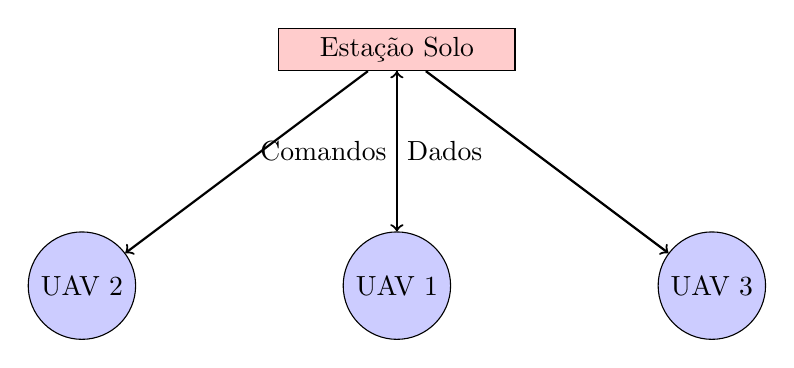
\begin{tikzpicture}[node distance=2cm]
    % Controlador Central
    \node[draw, rectangle, fill=red!20, minimum width=3cm] (central) {Estação Solo};
    % UAVs
    \node[draw, circle, fill=blue!20, below of=central, yshift=-1cm] (uav1) {UAV 1};  
    \node[draw, circle, fill=blue!20, left of=uav1, xshift=-2cm] (uav2) {UAV 2};  
    \node[draw, circle, fill=blue!20, right of=uav1, xshift=2cm] (uav3) {UAV 3};  
    % Conexões
    \draw[->, thick] (central) -- (uav1) node[midway, left] {Comandos};  
    \draw[->, thick] (central) -- (uav2);  
    \draw[->, thick] (central) -- (uav3);  
    \draw[->, thick, dashed] (uav1) -- (central) node[midway, right] {Dados};  
\end{tikzpicture}
    \caption{Arquitetura Centralizada.}
    \fonte{Elaborado pelo autor.}
    \label{fig:arquitetura_central}
\end{figure}

\begin{figure}[h]
    \centering
    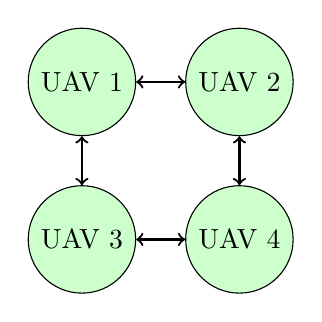
\begin{tikzpicture}[node distance=2cm]
    % UAVs
    \node[draw, circle, fill=green!20] (uav1) {UAV 1};  
    \node[draw, circle, fill=green!20, right of=uav1] (uav2) {UAV 2};  
    \node[draw, circle, fill=green!20, below of=uav1] (uav3) {UAV 3};  
    \node[draw, circle, fill=green!20, below of=uav2] (uav4) {UAV 4};  
    
    % Conexões peer-to-peer
    \draw[<->, thick] (uav1) -- (uav2);  
    \draw[<->, thick] (uav1) -- (uav3);  
    \draw[<->, thick] (uav2) -- (uav4);  
    \draw[<->, thick] (uav3) -- (uav4);  
\end{tikzpicture}
    \caption{Arquitetura Descentralizada.}
    \label{fig:arquitetura_desc}
\end{figure}


\begin{figure}[h]
    \centering
    \begin{tikzpicture}[node distance=3cm]
    % Central Planner
    \node[draw, rectangle, fill=orange!20] (central) {Estação Solo};
    % Subgroup Leaders
    \node[draw, diamond, fill=purple!20, below left of=central] (lider1) {Lider 1};  
    \node[draw, diamond, fill=purple!20, below right of=central] (lider2) {Lider 2};  
    % Planner connections
    \draw[->, dashed, thick] (central) -- (lider1);  
    \draw[->, dashed, thick] (central) -- (lider2);  
    % Subgroups
    \node[draw, circle, fill=cyan!20, below left of=lider1] (uav1) {UAV A};  
    \node[draw, circle, fill=cyan!20, right of=uav1] (uav2) {UAV B};
    \node[draw, circle, fill=cyan!20, right of=uav2] (uav3) {UAV C};  
    \node[draw, circle, fill=cyan!20, below right of=lider2] (uav4) {UAV D};  
    %\node[draw, circle, fill=cyan!20, left of=uav4] (uav5) {UAV E};  
    % Peer-to-peer connections
    \draw[<->, thick] (lider1) -- (uav1); 
    \draw[<->, thick] (lider1) -- (uav2);  
    \draw[<->, thick] (uav1) -- (uav2);  
    \draw[<->, thick] (lider2) -- (uav3);  
    \draw[<->, thick] (lider2) -- (uav4);
    \draw[<->, thick] (uav3) -- (uav4);
    \draw[<->, thick] (uav2) -- (uav3);  
\end{tikzpicture}
    \caption{Arquitetura Híbrida.}
    \fonte{Elaborado pelo autor.}
    \label{fig:arquitetura_hibrida}
\end{figure}


\subsection{Aplicações e Comportamentos de Enxames de UAVs}

Os enxames de UAVs têm ganhado destaque em diversas áreas devido à sua capacidade de realizar missões cooperativas de forma eficiente, robusta e escalável. Entre as principais aplicações, destacam-se as missões de vigilância e reconhecimento, como o rastreamento de alvos e patrulhamento de fronteiras, onde múltiplos drones podem cobrir grandes áreas simultaneamente, aumentando a efetividade da missão. Em situações de resposta a desastres, os enxames são empregados em tarefas de busca e resgate e avaliação de danos, oferecendo uma solução ágil e segura para operar em ambientes perigosos ou de difícil acesso.

Na agricultura de precisão, esses sistemas são utilizados para o monitoramento em larga escala de plantações, identificação de áreas afetadas por pragas ou falta de irrigação, bem como pulverização seletiva de pesticidas. Enxames também podem ser empregados como redes de comunicação móveis, oferecendo cobertura temporária de redes 5G ou 6G em áreas remotas ou durante eventos de emergência. Em operações militares, os UAVs em enxame são aplicados em ações coordenadas, como ataques simultâneos, guerra eletrônica, reconhecimento e bloqueio de sinais, com alto grau de adaptabilidade e redundância frente a ameaças.

A execução eficiente dessas aplicações depende de comportamentos cooperativos e distribuídos, que caracterizam os sistemas de enxame. Um dos comportamentos fundamentais é a formação de voo, onde os UAVs mantêm padrões geométricos estáveis — como formações em “V” ou em grade — permitindo maior organização e controle da missão. Outro comportamento essencial é a alocação de tarefas, que envolve a distribuição dinâmica de subtarefas entre os membros do enxame, frequentemente baseada em mecanismos de leilão, heurísticas distribuídas ou aprendizado por reforço.

O planejamento colaborativo de trajetórias e desvio de obstáculos garante que os UAVs naveguem de forma eficiente, evitando colisões e otimizando rotas em ambientes dinâmicos. A tomada de decisão coletiva é outro elemento-chave, permitindo que os drones cheguem a consensos em tempo real sobre alvos prioritários ou mudanças estratégicas na missão. Por fim, a autorreconfiguração é uma capacidade crítica de resiliência, na qual o enxame reorganiza sua estrutura e ajusta seu comportamento automaticamente em resposta à falha ou perda de um ou mais UAVs, assegurando a continuidade da operação.

Dessa forma, os enxames de UAVs oferecem um paradigma promissor para a automação de missões complexas, combinando aplicações práticas variadas com uma base de comportamentos coletivos sofisticados.

\subsection{Principais Desafios no Controle de Enxames VANTs}

O controle de enxames de UAVs envolve uma série de desafios técnicos e operacionais que precisam ser superados para garantir missões bem-sucedidas, especialmente em ambientes reais e dinâmicos. Um dos principais obstáculos está na complexidade da coordenação entre múltiplos agentes. Devido à observabilidade parcial, cada UAV frequentemente só tem acesso a informações limitadas sobre o ambiente e sobre os demais membros do enxame, o que restringe sua consciência situacional e dificulta a tomada de decisões cooperativas eficazes. Essa limitação é agravada pela não estacionariedade do ambiente, típica de cenários em que múltiplos agentes aprendem ou tomam decisões simultaneamente, interferindo uns nos outros.

Outro desafio crítico está relacionado à escalabilidade do sistema. À medida que o número de drones no enxame cresce, a comunicação entre os agentes tende a gerar uma sobrecarga significativa, cujo custo computacional e de largura de banda cresce quadraticamente com o tamanho do grupo. Além disso, a coordenação em espaços de ação conjuntos de alta dimensionalidade leva à chamada maldição da dimensionalidade, dificultando o planejamento e o aprendizado de políticas eficazes.

A atuação em ambientes dinâmicos e incertos impõe a necessidade de replanejamento constante. Obstáculos móveis, alterações nas condições ambientais e movimentação de alvos exigem que os UAVs adaptem suas trajetórias e estratégias de forma reativa e em tempo real. Nessas situações, incertezas associadas a medições de sensores ou limitações na precisão dos atuadores podem comprometer a segurança e a eficácia da missão.

As restrições físicas dos drones também impõem limitações operacionais significativas. A autonomia de voo é geralmente limitada pela capacidade das baterias, o que restringe o tempo de operação contínua. Além disso, o poder computacional embarcado costuma ser reduzido, exigindo algoritmos eficientes e leves para processamento local. Isso gera um constante trade-off entre exploração (busca por novas informações) e exploração (execução de ações já conhecidas como eficazes).

Por fim, aspectos relacionados à segurança e resiliência não podem ser negligenciados. UAVs estão sujeitos a vulnerabilidades como interferência eletromagnética, ataques de spoofing e ciberataques que podem comprometer o controle, a navegação ou a integridade dos dados. Em ambientes operacionais compartilhados, a presença de agentes adversários ou aeronaves desconhecidas representa uma ameaça adicional que deve ser considerada nos mecanismos de controle e decisão coletiva.

Esses desafios exigem abordagens inovadoras em áreas como aprendizado por reforço multiagente, controle distribuído, comunicações seguras e design de arquiteturas robustas para garantir que os enxames de UAVs possam operar de forma autônoma, eficiente e segura em cenários cada vez mais complexos.



\section{Fundamentos do Aprendizado por Reforço}

O Aprendizado por Reforço (Reinforcement Learning - RL) é um paradigma de aprendizado de máquina inspirado pela psicologia comportamental, onde um agente aprende a tomar decisões interagindo com um ambiente para maximizar recompensas cumulativas. Diferentemente do aprendizado supervisionado, no qual os modelos aprendem com dados rotulados, o RL depende de interações por tentativa e erro para descobrir estratégias ótimas. Segundo \cite{sutton2018reinforcement}, os conceitos fundamentais no RL são descritos como segue.
\begin{figure}[!h]
	\centering
	\includegraphics[scale=0.6]{fig/rl_loop_uav.png}
	\caption{Exemplo de diagrama esquemático sistema RL com agente VANT}
	\fonte{Autor.}
    \label{fig:rl_diagram}
\end{figure}

\subsection{Agente}
O agente é o tomador de decisões dentro do framework de RL. Ele interage com o ambiente executando ações e aprende uma política (\textit{policy})—um mapeamento entre estados e ações que determina a tomada de decisões do agente. A política é o núcleo central do agente, de modo esta determina o comportamento do agente. Portanto a fase de treinamento do agente, consiste em encontrar uma política que maximize a recompensa acumulada (retorno) esperada ao longo do período de atuação do agente.
A figura \ref{fig:rl_diagram} ilustra o fluxo de interação entre o agente e o ambiente. 
\subsection{Ambiente}
O ambiente representa tudo fora do agente com o qual ele interage. Ele fornece ao agente um estado ou observação, que é uma representação da situação atual que o agente é capaz de perceber, e responde às ações do agente mudando para um novo estado e oferecendo feedback em forma de recompensa. 
\begin{definition}[Framework RL]
Formalmente, o framwork de RL é modelado como um Processo de Decisão de Markov (MDP), definido pela tupla $\langle S,A,P,R \rangle$ onde:
\begin{itemize}
    \item (\(S\)): Conjunto denominado espaço de estados. Neste trabalho o espaço de estados são o conjunto de observações que o drone obtém do ambiente. Informações como: pose do drone no espaço, pontos de nuvem das leituras do sensor LiDAR, imagens das câmeras do drone, GPS (latitude e longitude).
    \item (\(A\)): Conjunto denominado espaço de ações.
    \item \(P(s_{t+1}|s_t, a_t)\): Uma função de transição , que define a probabilidade de transição para o estado \(s_{t+1}\) ao realizar a ação \(a_t\) no estado \(s_t\).
    \item \(R(s, a)\): Função de recompensa, que atribui um valor escalar às transições.
\end{itemize}
    
\end{definition}

\subsection{Recompensa}
A recompensa é um sinal de feedback escalar que quantifica o benefício imediato de uma ação tomada pelo agente. Este é o principal sinal que orienta o processo de aprendizado do agente. O objetivo do agente é maximizar a recompensa cumulativa (retorno) recebida ao longo do tempo. Isso envolve equilibrar recompensas imediatas e ganhos potenciais de longo prazo. O tipo de retorno mais utilizado é o \textbf{retorno esperado de horizonte infinito}, limitado o fator de desconto \(\gamma \in (0,1)\), definido como:
\begin{equation}
    R(\tau) = \sum_{t=0}^{\infty} \gamma^{t}r_t  
\end{equation}
onde $R(s_t, a_t)=r_t$ e $\tau=(s_0,a_0,s_1,a_1,...)$ representa um histórico de sequência de estados e ações tomadas no ambiente.
\subsection{Política}
A política (\(\pi\)) define o comportamento do agente. É uma função ou distribuição de probabilidade que mapeia estados para ações. Políticas podem ser determinísticas (\(a_t = \pi(s_t) \)) ou estocásticas \(\pi(a_t|s_t) \in [0,1]\).

\subsection{Problema central em RL}
O objetivo principal do aprendizado por reforço, consiste então, em selecionar uma política $\pi$ que maximize a função de retorno esperada. Para definir matematicamente esse problema é preciso estabelecer o conceito de trajetória, $\tau=(s_0,a_0,s_1,a_1,...) $ que representa uma sequência de estados e ações tomadas no ambiente. Então a probabilidade de uma trajetória é definido como:
\begin{equation}
    P(\tau|\pi)=\prod_{t=0}^{T} P(s_{t+1}|s_t, a_t)\pi(a_t,s_t)
\end{equation}
O retorno esperado para uma política específica $\pi$, é denotado por $J(\pi)$ definido como:
\begin{equation}
    J(\pi)=\int_{\tau}^{} P(\tau|\pi)R(\tau) \,d\tau  
\end{equation}
O problema central de otimização no aprendizado por reforço é modelado matematicamente então como:
\begin{equation}
    \pi^*=\arg \max_\pi J(\pi)
\end{equation}

\subsection{Funções de Valor}
As funções de valor avaliam a qualidade de estados ou pares estado-ação sob uma política dada, sendo fundamentais para orientar o agente a estratégias melhores:
\begin{itemize}
    \item Função de valor de estado \(V^\pi(s)=E\): Retorno esperado ao começar no estado \(s\) e seguir a política \(\pi\).
    \item Função de valor de ação (\(Q^\pi(s, a)\)): Retorno esperado ao tomar a ação \(a\) no estado \(s\) e seguir a política \(\pi\).
\end{itemize}

\subsection{Exploração versus Aprimoramento}
Um desafio fundamental no RL é o equilíbrio entre exploração (testar novas ações para descobrir seus efeitos) e aprimoramento (Exploitation) (escolher ações já conhecidas que maximizam recompensas). Estratégias como \(\epsilon\)-gananciosa (\(\epsilon\)-greedy) e Bound de Confiança Superior (UCB, do inglês Upper Confidence Bound) tratam deste equilíbrio ao combinar a necessidade do agente de coletar informações e alcançar altas recompensas.

\subsection{Métodos de Aprendizado}

Os algoritmos de Aprendizado por Reforço (Reinforcement Learning, RL) podem ser classificados em três grandes categorias, cada uma com diferentes estratégias para lidar com a dinâmica do ambiente e o processo de tomada de decisão.

Os métodos \textbf{model-free} (sem modelo) não exigem conhecimento prévio das funções de transição e recompensa do ambiente. Em vez disso, eles aprendem diretamente a política ou a função de valor a partir das interações com o ambiente. Dentro desta categoria, destacam-se os métodos baseados em valores, como o \textit{Q-Learning}, que busca estimar a função de valor de ação \( Q(s, a) \) para selecionar ações que maximizem a recompensa acumulada. Uma extensão poderosa dessa abordagem é o uso de redes neurais profundas, resultando nos \textit{Deep Q-Networks (DQNs)}, que permitem aplicar Q-Learning em ambientes com grandes espaços de estados, como aqueles representados por imagens ou sensores de alta dimensão.

Por outro lado, os métodos \textbf{model-based} (baseados em modelo) tentam construir uma representação explícita do ambiente, aprendendo suas dinâmicas — isto é, como os estados evoluem e quais recompensas são associadas às ações. Esses métodos permitem o uso de técnicas de planejamento, como simulações internas (\textit{rollouts}), para prever consequências futuras antes de agir, o que pode acelerar o processo de aprendizado e melhorar a amostragem de dados. Contudo, são mais sensíveis a erros no modelo aprendido.

A terceira categoria compreende os \textbf{métodos de otimização de política}, que consistem em atualizar diretamente os parâmetros da política com base em gradientes estimados da função objetivo. Ao invés de depender da estimativa de funções de valor, esses métodos otimizam diretamente a probabilidade de selecionar boas ações. Entre os algoritmos mais representativos dessa abordagem estão o \textit{Proximal Policy Optimization (PPO)} e o \textit{Trust Region Policy Optimization (TRPO)}, ambos amplamente utilizados por sua estabilidade e eficácia em tarefas com múltiplas etapas e ambientes contínuos.

Em sistemas multiagente, essas categorias se mantêm, mas a complexidade aumenta devido à não estacionariedade introduzida pela presença de múltiplos agentes aprendendo simultaneamente. A escolha do método adequado, portanto, deve considerar a natureza do ambiente, a escalabilidade e os objetivos do controle distribuído no sistema de enxame.


%Conforme discutido em \cite{sutton2018reinforcement}, o Aprendizado por Reforço tem sido amplamente aplicado em áreas como robótica, jogos e sistemas autônomos, destacando-se como uma abordagem poderosa, porém desafiadora, devido a problemas como recompensas esparsas e alta dimensionalidade de espaços de estado.

\section{Aprendizado por Reforço Multiagente (MARL)}
O Aprendizado por Reforço Multiagente (MARL) estende o aprendizado por reforço de agente único para ambientes onde múltiplos agentes aprendem a interagir e colaborar. 

\begin{definition}[Framework MARL]
Formalmente, o MARL é modelado como um \textbf{Jogo de Markov} \cite{LITTMAN}, definido pela tupla \(\langle \mathcal{N}, \mathcal{S}, \{\mathcal{A}^i\}, \mathcal{P}, \{\mathcal{R}^i\}, \gamma \rangle\), onde:
\begin{itemize}
    \item \(\mathcal{N}\): Conjunto de \(n\) agentes.
    \item \(\mathcal{S}\): Espaço de estados compartilhado.
    \item \(\mathcal{A}^i\): Espaço de ações do agente \(i\).
    \item \(\mathcal{P}(s' | s, \mathbf{a})\): Probabilidade de transição para o estado \(s'\) dada a ação conjunta \(\mathbf{a} = (a^1, \dots, a^n)\).
    \item \(\mathcal{R}^i(s, \mathbf{a})\): Função de recompensa do agente \(i\).
    \item \(\gamma\): Fator de desconto.
\end{itemize}
    
\end{definition}

Diferentemente do RL de agente único, no MARL os agentes devem equilibrar recompensas individuais com objetivos coletivos, gerando desafios únicos:
\begin{itemize}
    \item \textbf{Não Estacionariedade}: Políticas dos agentes mudam concorrentemente, violando a suposição de Markov.%\cite{foerster2017stabilising}.
    \item \textbf{Atribuição de Crédito}: Dificuldade em associar sucessos/falhas globais a ações individuais.% \cite{wei2021credit}.
    \item \textbf{Observabilidade Parcial}: Agentes observam apenas estados locais \(o^i \subset \mathcal{S}\).% \cite{oliehoek2016concise}.
\end{itemize}

\subsection{Abordagens Algorítmicas em MARL}  
Os desafios de coordenação em enxames de UAVs exigem estratégias de \textit{Multi-Agent Reinforcement Learning} (MARL) que equilibrem escalabilidade, eficiência e adaptabilidade. A literatura especializada propõe três paradigmas principais para lidar com essas demandas:  
\begin{enumerate}
    \item \textbf{Aprendizado Independente (IQL - Independent Q-Learning)} \cite{tan1993multi}:  
    Nesta abordagem, cada agente aprende uma função de valor \(Q^i(o^i, a^i)\) de forma totalmente descentralizada, ignorando as ações e observações dos demais. A simplicidade computacional do IQL o torna escalável para grandes enxames, mas a falta de modelagem explícita das interdependências entre agentes frequentemente resulta em coordenação subótima, especialmente em tarefas que exigem sincronização ou divisão de recursos \cite{tan1993multi}.  
    
    \item \textbf{Treinamento Centralizado com Execução Descentralizada (CTDE)} \cite{kraemer2016multi}:  
    Para superar as limitações do IQL, métodos como o QMIX 
    utilizam informações globais durante o treinamento (e.g., estados agregados do enxame) enquanto mantêm políticas de execução baseadas em observações locais. O QMIX, por exemplo, impõe uma fatorização monotônica das funções-Q individuais (\( \partial Q_{\text{total}} / \partial Q^i \geq 0 \)), garantindo que a maximização dos Q-valores locais corresponda à otimização do valor global do enxame. Essa estratégia é particularmente eficaz em missões de vigilância cooperativa, onde a coordenação tácita é crítica \cite{rashid2018qmix}.  

    \item \textbf{Treinamento e Execução Totalmente Descentralizados (DTDE)} \cite{schulman2017}:  
    Algoritmos como o IPPO (\textit{Independent Proximal Policy Optimization}) priorizam a escalabilidade extrema, permitindo que cada agente treine e execute políticas baseadas apenas em observações locais. Embora adequado para enxames massivos em ambientes com restrições de comunicação, o DTDE enfrenta dificuldades em cenários que exigem sincronização fina entre agentes, como formação dinâmica em espaços congestionados \cite{schulman2017}.  

\end{enumerate}

Dentre os algoritmos de Aprendizado por Reforço Multiagente (MARL) mais consolidados para controle de enxames, destacam-se:

\begin{itemize}
    \item \textbf{MAPPO} \cite{yu2021mappo}: Baseado no paradigma CTDE (Centralized Training with Decentralized Execution), combina redes \textit{actor-critic} com críticos centralizados, sendo especialmente eficaz em espaços de ação contínuos — ideal para ajustes precisos de trajetória em UAVs.
    
    \item \textbf{VDN} \cite{sunehag2017value}: Decompõe o valor global do enxame em uma soma de Q-valores individuais, o que facilita a otimização distribuída em tarefas como a cobertura eficiente de áreas.
    
    \item \textbf{Mean-Field MARL} \cite{yang2018mean}: Modela as interações entre agentes como a média do comportamento coletivo, reduzindo significativamente a complexidade computacional — uma abordagem eficaz em cenários envolvendo centenas de UAVs.
\end{itemize}

Apesar dos avanços recentes, diversos desafios práticos ainda persistem. Algoritmos CTDE, como o QMIX, demandam comunicação de alta frequência durante o treinamento, o que limita sua aplicabilidade em sistemas com restrições energéticas \cite{rashid2018qmix}. Por outro lado, abordagens totalmente descentralizadas (DTDE) enfrentam a ``maldição da dimensionalidade'', especialmente em ambientes parcialmente observáveis \cite{schulman2017}. Além disso, a maioria das validações ocorre em simulações homogêneas, enquanto aplicações reais introduzem variabilidades como heterogeneidade de sensores, atrasos de comunicação e falhas de hardware não modeladas \cite{yang2018mean}.

Nesse contexto, a integração de MARL com técnicas de \textit{transfer learning} e arquiteturas neuro-simbólicas desponta como uma estratégia promissora para superar essas limitações e aproximar a pesquisa do uso prático em campo.


\subsection{Multi-Agent Proximal Policy Optimization (MAPPO)}
\label{subsec:mappo}

O \textit{Multi-Agent Proximal Policy Optimization} (MAPPO) é um algoritmo de aprendizado por reforço multiagente que estende o método \textit{Proximal Policy Optimization} (PPO), proposto originalmente por Schulman et al.~\cite{schulman2017ppo}, para cenários cooperativos com múltiplos agentes. O MAPPO foi formalizado por Yu et al.~\cite{yu2021mappo} como uma alternativa estável e escalável para problemas caracterizados por observabilidade parcial e necessidade de coordenação, como aqueles encontrados em sistemas de enxames de veículos aéreos não tripulados.

O MAPPO adota o paradigma de \textit{Centralized Training with Decentralized Execution} (CTDE), no qual o treinamento das políticas é realizado de forma centralizada, enquanto a execução ocorre de maneira descentralizada. Nesse contexto, cada agente executa uma política local baseada apenas em suas observações individuais, ao passo que, durante o treinamento, um crítico centralizado pode explorar informações globais do sistema para estimar funções de valor mais informativas, reduzindo a variância das atualizações de política.

Considere um sistema composto por $N$ agentes. Cada agente $i$ observa, no instante $t$, uma observação local $\mathbf{o}_i(t)$ e executa uma ação $\mathbf{a}_i(t)$ de acordo com uma política estocástica parametrizada $\pi_\theta$, compartilhada entre todos os agentes:
\[
\mathbf{a}_i(t) \sim \pi_\theta(\mathbf{a}_i \mid \mathbf{o}_i).
\]
O compartilhamento de parâmetros entre agentes, prática adotada no MAPPO, contribui para a escalabilidade do algoritmo e para a emergência de comportamentos cooperativos simétricos~\cite{yu2021mappo}.

Durante o treinamento, o MAPPO emprega um crítico centralizado $V_\phi$, que estima o valor esperado do retorno a partir de um estado global ou de uma concatenação das observações dos agentes:
\[
V_\phi(\mathbf{s}(t)) \approx \mathbb{E}\!\left[ \sum_{k=0}^{\infty} \gamma^k r(t+k) \,\middle|\, \mathbf{s}(t) \right],
\]
onde $\mathbf{s}(t)$ representa o estado global disponível apenas durante o treinamento, $r(t)$ é a recompensa compartilhada e $\gamma \in (0,1)$ é o fator de desconto.

O MAPPO herda do PPO a função objetivo baseada em \textit{clipping}, projetada para limitar variações excessivas na política durante as atualizações e garantir estabilidade no processo de aprendizado~\cite{schulman2017ppo}. A função objetivo otimizada pelo ator é dada por:
\[
\mathcal{L}^{\text{CLIP}}(\theta) =
\mathbb{E}_t \left[
\min \left(
\rho_t(\theta) \hat{A}_t,\;
\mathrm{clip}\big(\rho_t(\theta), 1-\epsilon, 1+\epsilon\big)\hat{A}_t
\right)
\right],
\]
em que $\rho_t(\theta) = \frac{\pi_\theta(\mathbf{a}_i(t)\mid \mathbf{o}_i(t))}{\pi_{\theta_{\text{old}}}(\mathbf{a}_i(t)\mid \mathbf{o}_i(t))}$ é a razão de probabilidade entre a política atual e a anterior, $\epsilon$ é o parâmetro de \textit{clipping} e $\hat{A}_t$ representa a estimativa da vantagem.

A estimativa da vantagem é tipicamente calculada por meio do método de \textit{Generalized Advantage Estimation} (GAE), introduzido por Schulman et al.~\cite{schulman2016gae}, que combina viés e variância de forma controlada:
\[
\hat{A}_t = \sum_{l=0}^{\infty} (\gamma \lambda)^l \delta_{t+l},
\quad
\delta_t = r(t) + \gamma V_\phi(\mathbf{s}(t+1)) - V_\phi(\mathbf{s}(t)),
\]
onde $\lambda \in (0,1)$ é o parâmetro de suavização temporal.

Ao combinar a estabilidade do PPO com o formalismo CTDE, o MAPPO fornece uma abordagem robusta para aprendizado por reforço multiagente em ambientes contínuos e parcialmente observáveis, sendo amplamente adotado em tarefas cooperativas complexas, incluindo controle de formações e coordenação de enxames robóticos~\cite{yu2021mappo}.

\begin{figure}[H]
\centering
\begin{tikzpicture}[
    node distance=1.2cm and 2.4cm,
    actor/.style={rectangle, draw, fill=blue!15, minimum width=3.2cm, minimum height=0.9cm, align=center},
    critic/.style={rectangle, draw, fill=red!15, minimum width=3.2cm, minimum height=0.9cm, align=center},
    env/.style={rectangle, draw, fill=green!15, minimum width=3.2cm, minimum height=0.9cm, align=center},
    buffer/.style={rectangle, draw, fill=gray!15, minimum width=3.2cm, minimum height=0.9cm, align=center},
    update/.style={rectangle, draw, fill=yellow!20, minimum width=3.2cm, minimum height=0.9cm, align=center},
    arrow/.style={->, thick},
    dashedarrow/.style={->, thick, dashed},
    every node/.style={font=\footnotesize}
]

% Nodes
\node[actor] (actor) {Shared Actor\\$\pi_\theta(\mathbf{a}_i \mid \mathbf{o}_i)$};

\node[env, below=of actor] (env) {Multi-Agent Environment};

\node[critic, right=of env] (critic) {Centralized Critic\\$V_\phi(\mathbf{s})$};

\node[buffer, below=of env] (buffer) {Trajectory Buffer};

\node[update, below=of buffer] (update) {PPO + GAE\\Update};

% Execution flow
\draw[arrow] (actor) -- node[left] {local actions $\mathbf{a}_i$} (env);
\draw[arrow] (env) -- node[left] {local obs $\mathbf{o}_i$} (actor);

% Centralized training flow
\draw[arrow] (env) -- node[above] {global state $\mathbf{s}$} (critic);
\draw[arrow] (critic) -- node[right] {value estimates} (buffer);

\draw[arrow] (env) -- node[left] {trajectories} (buffer);

\draw[arrow] (buffer) -- node[left] {advantages} (update);

\draw[dashedarrow] (update.west) -| node[above] {policy \& value update} (actor.west);
\draw[dashedarrow] (update.east) -| (critic.east);

% Labels
\node[above=0.4cm of actor] {\textbf{Decentralized Execution}};
\node[right=0.2cm of critic] {\textbf{Centralized Training}};

\end{tikzpicture}
\caption{Fluxograma do treinamento MAPPO no paradigma de Treinamento Centralizado com Execução Descentralizada (CTDE). Durante a execução, cada agente utiliza apenas observações locais por meio de uma política compartilhada. Durante o treinamento, um crítico centralizado explora o estado global para atualizar os parâmetros da política e da função de valor.}
\label{fig:ctde_flow}
\end{figure}

\subsection{Descrição Algorítmica do MAPPO}

O Algoritmo~\ref{algo:mappo} apresenta o fluxo geral de treinamento do MAPPO no paradigma de \textit{Centralized Training with Decentralized Execution} (CTDE). Durante a coleta de experiências, cada agente executa ações de forma descentralizada a partir de observações locais, utilizando uma política compartilhada entre todos os agentes. Em contrapartida, a atualização dos parâmetros é realizada de forma centralizada, explorando um crítico global que tem acesso ao estado conjunto do sistema.

A interação com o ambiente gera trajetórias multiagentes compostas por observações locais, ações e recompensas compartilhadas, que são armazenadas em um buffer de experiências. A partir dessas trajetórias, são estimadas as vantagens utilizando o método de \textit{Generalized Advantage Estimation} (GAE). O ator é então atualizado por meio da função objetivo com \textit{clipping} do PPO, enquanto o crítico é otimizado por regressão sobre o retorno esperado.

Esse procedimento permite reduzir a variância das atualizações de política, ao mesmo tempo em que preserva a execução descentralizada, característica fundamental para aplicações em sistemas distribuídos, como enxames de VANTs.

\begin{algorithm}[H]
\caption{Multi-Agent Proximal Policy Optimization (MAPPO)}
\label{algo:mappo}
\begin{algorithmic}[1]
\STATE Inicializar política compartilhada $\pi_\theta$ e crítico centralizado $V_\phi$
\FOR{episódio = $1$ até $N_{\text{episódios}}$}
    \STATE Inicializar ambiente multiagente
    \STATE Inicializar buffer de trajetórias $\mathcal{B} \leftarrow \emptyset$
    \FOR{passo = $1$ até $T$}
        \FOR{cada agente $i = 1,\dots,N$}
            \STATE Observar estado local $\mathbf{o}_i(t)$
            \STATE Amostrar ação $\mathbf{a}_i(t) \sim \pi_\theta(\cdot \mid \mathbf{o}_i(t))$
        \ENDFOR
        \STATE Executar ação conjunta $\mathbf{a}(t)$ no ambiente
        \STATE Obter recompensa compartilhada $r(t)$ e novas observações
        \STATE Armazenar $(\mathbf{o}(t), \mathbf{a}(t), r(t), \mathbf{o}(t+1))$ em $\mathcal{B}$
    \ENDFOR
    \STATE Estimar vantagens $\hat{A}_t$ usando GAE
    \FOR{época de atualização = $1$ até $K$}
        \STATE Atualizar crítico: $\phi \leftarrow \phi - \alpha_V \nabla_\phi \mathcal{L}_V$
        \STATE Atualizar ator via PPO:
        \[
        \theta \leftarrow \theta - \alpha_\pi \nabla_\theta 
        \mathbb{E}\big[\min(\rho_t \hat{A}_t,
        \mathrm{clip}(\rho_t,1-\epsilon,1+\epsilon)\hat{A}_t)\big]
        \]
    \ENDFOR
\ENDFOR
\end{algorithmic}
\end{algorithm}




%\subsection{MARL para Enxames de VANTs}
%O MARL é particularmente adequado para controle de enxames de UAVs devido à sua capacidade de:
%\begin{itemize}
%    \item Escalar para grandes populações de agentes via treinamento e execução descentralizada (\textit{Decentralized Training and Decentralized Execution} - DTDE).
%    \item Otimizar objetivos globais (ex: rastreamento de alvos) através de coordenação emergente.
%    \item Adaptar-se a ambientes dinâmicos via aprendizado online.
%\end{itemize}


\section{Máquinas de Recompensa}

\subsection{Conceitos sobre RMs}

As \textit{Reward Machines} (RMs) consistem em um formalismo baseado em autômatos finitos que visa estruturar e modularizar funções de recompensa em problemas de aprendizado por reforço (RL). Tradicionalmente, as funções de recompensa são tratadas como "caixas-pretas", sendo acessadas pelo agente apenas para consulta pontual de valores. As RMs propõem uma abordagem diferente, em que a estrutura interna da função de recompensa é explicitada ao agente, permitindo que ele utilize tal conhecimento para acelerar e modular o processo de aprendizado \cite{rm_marl}.

\begin{definition}[Máquina de Recompensas]
Uma \textbf{Reward Machine} (RM) é uma tupla $M = \langle U, u_0, F, \delta_u, \delta_r, P \rangle$, onde:
\begin{itemize}
    \item $U$ é um conjunto finito de estados da máquina de recompensa;
    \item $u_0 \in U$ é o estado inicial da RM;
    \item $F \subseteq U$ é o conjunto de estados terminais;
    \item $P$ é um conjunto de proposições que descrevem eventos observáveis no ambiente;
    \item $\delta_u : U \times 2^{P} \rightarrow U \cup F$ é a função de transição da RM, que define a mudança de estados da RM com base nos eventos observados;
    \item $\delta_r : U \times 2^{P} \rightarrow \mathbb{R}$ é a função de recompensa que associa uma recompensa real a cada transição da RM.
\end{itemize}
\end{definition}


Formalmente, uma RM é composta por um conjunto de estados $U$, uma função de transição $\delta_u$, e uma função de recompensa $\delta_r$. O agente, ao interagir com o ambiente, transita não apenas pelos estados do ambiente, mas também pelos estados da RM, de acordo com eventos de alto nível observados no ambiente e definidos via uma função de rotulagem $L$. Cada transição na RM pode especificar uma recompensa distinta, tornando possível descrever recompensas não-Markovianas ou recompensas que dependem de propriedades temporais do histórico do agente.




A principal vantagem das RMs está na capacidade de decompor missões complexas em \textit{subtarefas} modulares, facilitando a especificação de propriedades temporais como sequências de eventos, loops e condicionais. Por exemplo, em um cenário de entrega de pacotes com UAVs, uma RM pode especificar que primeiro o agente deve "localizar o alvo" e, em seguida, "entregar o pacote" em outra localização, premiando adequadamente cada etapa.

%Além de aumentar a expressividade da função de recompensa, as RMs possibilitam a aplicação de técnicas de \textit{shaping} de recompensas e decomposição hierárquica de políticas. Técnicas como Q-learning para RMs (QRM) ou abordagens de \textit{counterfactual reasoning} (CRM) se beneficiam diretamente da estrutura exposta pelas RMs, resultando em melhor eficiência amostral e políticas mais robustas em ambientes parcialmente observáveis ou com recompensas esparsas.

Por fim, as RMs possuem o mesmo poder expressivo de linguagens regulares, sendo capazes de capturar propriedades temporais similares às especificadas por lógicas como LTL (\textit{Linear Temporal Logic}), oferecendo uma alternativa prática e compacta para a especificação de tarefas em RL.

\begin{definition}[MDP com Reward Machine (MDPRM)]
Um \textbf{MDP com Reward Machine} é uma tupla estendida $T = \langle S, A, p, \gamma, P, L, M \rangle$, onde:
\begin{itemize}
    \item $S$ é o conjunto finito de estados do ambiente;
    \item $A$ é o conjunto finito de ações disponíveis ao agente;
    \item $p: S \times A \times S \rightarrow [0,1]$ é a função de transição estocástica do ambiente;
    \item $\gamma \in (0,1]$ é o fator de desconto;
    \item $P$ é o conjunto de proposições de eventos (compartilhado com a RM);
    \item $L : S \times A \times S \rightarrow 2^{P}$ é a função de rotulagem, que associa a cada transição no ambiente um conjunto de proposições verdadeiras;
    \item $M = \langle U, u_0, F, \delta_u, \delta_r, P \rangle$ é a \textit{Reward Machine} associada.
\end{itemize}
\end{definition}

\begin{figure}[H]
    \centering
    \begin{tikzpicture}[->, >=stealth', node distance=3cm, auto, thick, align=center]
        % Ambiente
        \node[draw, rectangle, rounded corners, minimum width=3.5cm, minimum height=1cm] (env) {Ambiente (MDP) \\ $s_t \xrightarrow{a_t} s_{t+1}$};

        % Label function
        \node[draw, ellipse, right of=env, node distance=4.5cm] (label) {Rotulagem \\ $\sigma_t = L(s_t, a_t, s_{t+1})$};

        % Reward Machine
        \node[draw, rectangle, rounded corners, right of=label, node distance=4.5cm, minimum width=3.5cm, minimum height=1cm] (rm) {Reward Machine \\ $u_t \xrightarrow{\sigma_t} u_{t+1}$};

        % Reward output
        \node[draw, rectangle, below of=rm, node distance=2.5cm, minimum width=3cm] (reward) {Recompensa $r_t$};

        % Arrows
        \path (env) edge node[above] {} (label);
        \path (label) edge node[above] {} (rm);
        \path (rm) edge node[right] {} (reward);

        % Feedback loop to agent (optional)
       % \draw[->, dashed] (reward.west) to[out=180,in=-90] node[left] {Reforço para o agente} ([yshift=-1cm]env.south);

    \end{tikzpicture}
    \caption{Fluxo de interação entre o ambiente, a função de rotulagem e a Reward Machine.}
    \fonte{Adapatado de \cite{rm_marl}}
    \label{fig:mdprm}
\end{figure}
A figura \ref{fig:mdprm} ilustra como a função de rotulagem $L$ realiza a interface entre a transição dos estados do ambiente com a transição de estados da máquina de recompensa. O agente ao realizar a ação $a_t$ muda o estado do ambiente de $s_t $ para $s_{t+1}$. A função rotulagem $L$ transforma a 3-tupla $(s_t,a_t,s_{t+1})$ em uma transição $\sigma_t$ da máquina de recompensa alterando seu estado de $u_t$ para $u_{t+1}$, fornecendo a recompensa $r_t$ para o agente.
\subsection{Exemplo RM: Grid World}
\begin{figure}[!h]
	\centering
	\includegraphics[scale=0.9]{fig/RM_grid_world.png}
	\caption{Exemplo de RM para o ambiente GridWorld}
	\fonte{Extraído de \cite{rm_marl}}
    \label{fig:rm_grid}
\end{figure}
A figura \ref{fig:rm_grid} mostra um exemplo de máquina de recompensas para o ambiente \textit{GridWorld}. Neste ambiente o agente consegue se movimentar nas direções cardinais, seu objetivo consiste em obter o café e o jornal acessando as posições em que os itens se encontram e entrega-las até a posição do escritório $o$. Este é um exemplo simples no qual há um requisito temporal para as sequências das atividades que o agente deve completar antes de chegar até o seu destino final. Os rótulos sobre as setas de transições da máquina de recompensa na figura a direita indicam em forma de 2-tupla respectivamente a função de rotulagem e o retorno esperado pelo agente. Por exemplo o sob o estado $u_1$ o rótulo $<\neg o \land \neg*,0>$ indica que quando o agente movimenta-se para uma posição que não é o escritório $(o)$ e também não possui um obstáculo $(*)$ ele recebe a recompensa escalar 0 e mantém a máquina de estados no estado $u_1$.